%%%%%%%%%%%%%%%%%%%%%%%%%%%%%%%%%%%%%%%%%%%%%%%%%%%%%%%%%%%%%%%%%%%%
% HEALTHINFO IV -- Track B
% Chu de: Health Literacy (tru cot 6)
%
% GHI CHU CHO TAC GIA:
%  - Ban dang nop review DOUBLE-BLIND: giu nguyen phan \author va
%    \institute an danh o duoi. Chi dien ten that o ban camera-ready.
%  - Abstract Springer yeu cau 70-150 tu. Trang Call for Papers ghi 300 tu.
%    Da hoi BTC; hien dang viet theo chuan Springer (150 tu).
%%%%%%%%%%%%%%%%%%%%%%%%%%%%%%%%%%%%%%%%%%%%%%%%%%%%%%%%%%%%%%%%%%%%

\documentclass{svproc}

\usepackage{url}
\def\UrlFont{\rmfamily}
\usepackage[utf8]{inputenc}
\usepackage[T1]{fontenc}
\usepackage{booktabs}
\usepackage{graphicx}
\usepackage{amsmath}

% Tranh de LaTeX day hinh sang mot trang rieng gan nhu trong (thua khong
% gian). Chi anh huong cach dat float, khong doi noi dung.
\renewcommand{\textfraction}{0.05}
\renewcommand{\topfraction}{0.95}
\renewcommand{\bottomfraction}{0.9}
\renewcommand{\floatpagefraction}{0.75}
\setcounter{topnumber}{3}
\setcounter{bottomnumber}{2}
\setcounter{totalnumber}{4}
\setlength{\intextsep}{8pt plus 2pt minus 2pt}
\setlength{\textfloatsep}{10pt plus 2pt minus 2pt}

\begin{document}
\mainmatter

\title{A Rule-Constrained Large Language Model Pipeline for
Patient-Friendly Interpretation of Vietnamese Blood Test Results}

\titlerunning{Rule-Constrained LLM for Blood Test Interpretation}

% === AN DANH CHO VONG PHAN BIEN ===
\author{Anonymous Author(s)}
\authorrunning{Anonymous}
\institute{Anonymous Institution}

% === BAN CAMERA-READY: bo comment cac dong duoi, xoa 3 dong tren ===
% \author{Vo Hoang Khang}
% \authorrunning{V. H. Khang}
% \institute{HUTECH University, Ho Chi Minh City, Vietnam,\\
% \email{...}}

\maketitle

\begin{abstract}
Patients in Vietnam routinely receive laboratory reports written in
clinical terminology they cannot interpret, and increasingly turn to
general-purpose language models for explanations. We show this is unsafe:
an unconstrained model asked to explain synthetic complete blood count
panels misstated the direction of an analyte in 91.3\% of cases and told
patients with abnormal results that everything was normal in 32.0\% of
cases. We propose a four-layer pipeline in which all clinical judgement is
made by deterministic rules before the language model is invoked; the model
only paraphrases pre-assigned labels, and a post-generation validator
rejects outputs that contradict them. On 150 synthetic panels, the full
pipeline produced no unsafe output, with 64.0\% generated by the model and
36.0\% falling back to fixed templates. The system runs on CPU without a GPU.
\keywords{health literacy, large language models, laboratory results,
patient communication, AI safety}
\end{abstract}


%%%%%%%%%%%%%%%%%%%%%%%%%%%%%%%%%%%%%%%%%%%%%%%%%%%%%%%%%%%%%%%%%%%%
\section{Introduction}
%%%%%%%%%%%%%%%%%%%%%%%%%%%%%%%%%%%%%%%%%%%%%%%%%%%%%%%%%%%%%%%%%%%%

A patient leaving a Vietnamese laboratory receives a printed panel of
numbers annotated with terms such as \texttt{PDW}, \texttt{MCHC}, and
\texttt{Monocyte}, in units of \texttt{G/L}, \texttt{fL}, and \texttt{pg}.
The reference interval is printed beside each value, so a patient can see
that a number falls outside it, but not what the analyte measures, whether
the deviation matters, or what to do next. The gap between possessing a
result and understanding it is what health literacy describes: the
ability to access, understand, appraise, and use health information to
maintain one's health.

That patients are left to close this gap alone is documented: in a study of
93 patients receiving results through an online portal, nearly two-thirds
received no explanation of their results and 46\% searched online to
understand them~\cite{giardina2018perceptions}. Increasingly, that search
means photographing the report and asking a general-purpose language
model --- a failure mode easy to reproduce: asked in Vietnamese what white
blood cells are, the 3B-parameter model used in this study replied that
they are lymphocytes (one type of white blood cell, not a synonym) and,
unprompted, mentioned cancer and immune deficiency, handing an ordinary
result a definitional error and two alarming diseases in one short answer.

The more consequential failure runs in the opposite direction. A model
that summarises an abnormal panel as normal does not merely misinform; it
removes the reason to seek care. Terminological errors are visible and
invite verification, whereas false reassurance is fluent, comfortable, and
acts by suppressing further action, so we treat it as a distinct error
class and measure it separately: an unconstrained model produced it on
32.0\% of abnormal panels in our data.

Our position is that the task should not be given to the model in the form
it usually is. Deciding whether a value is abnormal is arithmetic against
a reference interval, which a program does exactly; rendering that
determination in plain language is what a language model does well.
Separating the two, and verifying the second against the first, removes
the failure mode rather than instructing it away.

This paper contributes:

\begin{enumerate}
\item A four-layer pipeline in which all clinical judgement is completed
by deterministic rules before generation, so the model paraphrases
pre-assigned labels rather than deriving them.
\item An automated post-generation validator that checks generated text
against those labels and falls back to fixed templates when it does not
agree, so that no unverified text reaches the reader.
\item An evaluation on 150 synthetic complete blood count panels
measuring six error classes, including false reassurance, which to our
knowledge has not been reported separately in prior work on patient-facing
result explanation.
\item An observation that unit heterogeneity between Vietnamese
laboratories introduces severe misclassification inside the rule layer
itself unless explicitly normalised.
\end{enumerate}


%%%%%%%%%%%%%%%%%%%%%%%%%%%%%%%%%%%%%%%%%%%%%%%%%%%%%%%%%%%%%%%%%%%%
\section{Related Work}
%%%%%%%%%%%%%%%%%%%%%%%%%%%%%%%%%%%%%%%%%%%%%%%%%%%%%%%%%%%%%%%%%%%%

\subsection{Language Models for Patient-Facing Result Explanation}

The closest prior work evaluates whether general-purpose models can answer
patients' questions about laboratory results. He et al.~\cite{he2024quality}
compared model responses against peer answers on 53 forum question--answer
pairs, assessing relevance, accuracy, helpfulness, and harmfulness, with
GPT-4 outperforming smaller open models; related radiology
work~\cite{llm_radiology_explain} measured readability, understandability,
and anxiety-inducing potential across several models.

Assessments from within laboratory medicine are more cautious. The
European Federation of Clinical Chemistry and Laboratory Medicine working
group on artificial intelligence reported that such models may give
superficial or incorrect answers to questions about test results and
concluded they cannot be used for diagnosis~\cite{cadamuro2023eflm}. On 30
interpretation questions posed by physicians, GPT-4 answered 46.7\%
correctly, gave partially correct answers to 23.3\%, and answered 30\%
incorrectly or irrelevantly~\cite{munoz2023accuracy}. These evaluations
concern clinicians as users; the patient-facing case is more exposed,
since the reader has less basis for recognising an incorrect answer.

Two features of this literature motivate our approach. Evaluation is
oriented towards readability and general accuracy; harmfulness, where
assessed, is one dimension among several rather than decomposed into
specific failure modes, and we are not aware of prior work that isolates
false reassurance despite its distinctive consequence of suppressing
care-seeking. Moreover, these studies evaluate models directly, without a
mechanism to stop an unsafe response reaching the reader. Our contribution
is architectural rather than evaluative: not how well a model performs the
task, but how to arrange the system so its failures do not propagate.

\subsection{Health Literacy in Vietnam}

The premise that patients cannot interpret their own laboratory reports is
well supported in the Vietnamese context. A cross-sectional study of 204
older adults in Da Nang found 60.3\% with inadequate general health
literacy, with urban residents scoring 2.4 times higher than rural ones
and educational attainment a strong determinant~\cite{danang2025older}.
Earlier work reported similar patterns~\cite{duong2020elderly,hlq_vietnam2025}.
A recent national survey reports a combination directly relevant here:
high eHealth literacy alongside low general health literacy among
digitally connected adults, with online health-seeking behaviour
common~\cite{ehealth_literacy_vn2026}. Patients are therefore willing to
consult online tools while less equipped to evaluate them --- raising,
not lowering, the safety requirement on such tools.

\subsection{Constraining and Verifying Model Output}

Grammar-constrained decoding restricts the token distribution at each step
so that only strings conforming to a grammar can be
produced~\cite{geng2023grammar,willard2023outlines}, and schema-constrained
generation is now a standard interface for machine-readable output.

Structural validity, however, does not entail semantic correctness: a
response may satisfy a schema exactly while containing values that are
wrong for the input. Our Layer~4 operates at this second level. It does
not check that the output parses --- the schema constraint already
ensures that --- but that its content agrees with labels computed
independently of the model. This is closer to verification against an
external source of truth than to constrained decoding, and the two are
complementary: we apply schema constraints at generation time and semantic
verification afterwards.

\subsection{Laboratory Data and Unit Standardisation}

The unit inconsistency we encountered is known at larger scale. Between
6\% and 19\% of laboratory tests cannot be accurately mapped to LOINC,
with missing or incorrect units among the recurring
obstacles~\cite{loinc_harmonize2026}, and an analysis of over 163 million
LOINC-mapped results identified 2{,}019 distinct unit expressions, reduced
by harmonisation to roughly 40 reference units~\cite{unit_harmonize2025}.
Automated mapping approaches exist for codes~\cite{mcdonald2018loinc}.

This literature treats unit heterogeneity as an obstacle to data
aggregation and secondary analysis. Our observation is that it is also a
patient-safety issue: within our pipeline, comparing an unconverted value
against a reference interval in a different unit produced a severe
misclassification of a normal result, inside the deterministic layer the
architecture relies on for correctness. The argument for standardisation
is usually made in terms of research reuse; we offer a small piece of
evidence that it also bears on what a patient is told about their own
results.


%%%%%%%%%%%%%%%%%%%%%%%%%%%%%%%%%%%%%%%%%%%%%%%%%%%%%%%%%%%%%%%%%%%%
\section{System Design}
%%%%%%%%%%%%%%%%%%%%%%%%%%%%%%%%%%%%%%%%%%%%%%%%%%%%%%%%%%%%%%%%%%%%

The central design principle is that \emph{no clinical judgement is
delegated to the language model}. Whether an analyte is abnormal, and how
severely, is decided by deterministic rules before the model is invoked.
The model receives values that have already been labelled and is asked only
to paraphrase them. A post-generation validator then checks that the
generated text is consistent with those labels, and the system falls back
to fixed templates when it is not.

Figure~\ref{fig:arch} shows the four layers.

\begin{figure}[htbp]
\centering
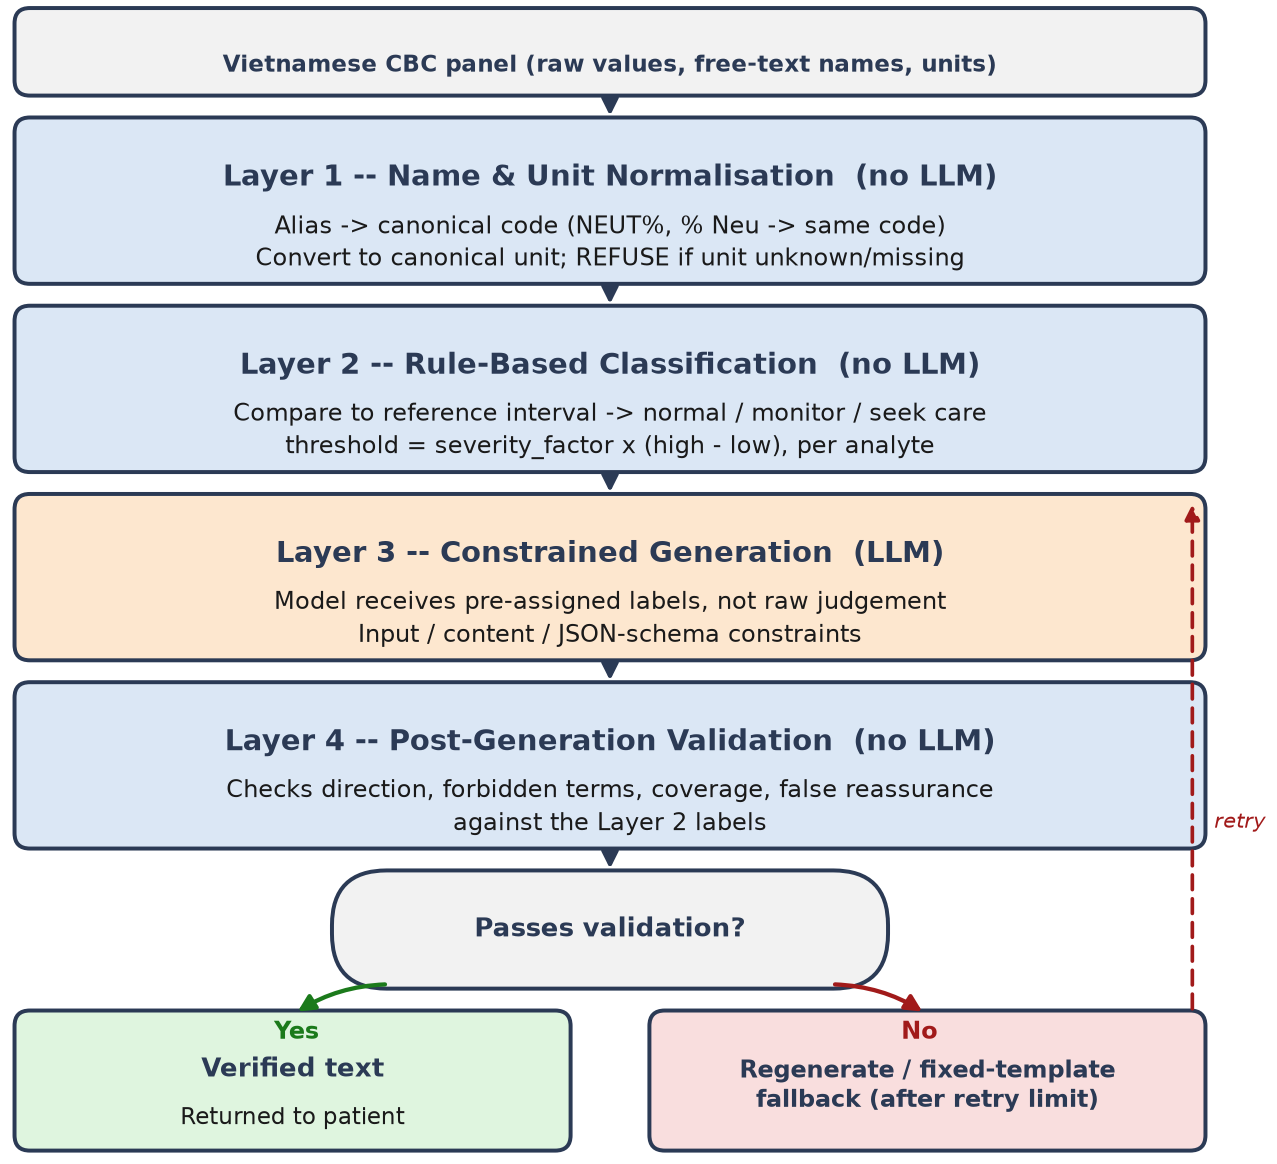
\includegraphics[width=0.98\textwidth]{architecture.png}
\caption{Four-layer pipeline. Clinical judgement (Layer~2) precedes
generation (Layer~3); Layer~4 verifies the output against Layer~2's
labels.}
\label{fig:arch}
\end{figure}

\subsection{Layer 1: Name and Unit Normalisation}

Vietnamese laboratories name the same analyte inconsistently: a white
blood cell count may appear as \texttt{WBC}, the Vietnamese abbreviation
\texttt{SLBC}, the full Vietnamese phrase, or \texttt{* WBC}. Percentage
and absolute counts are distinguished only by a \texttt{\%} or \texttt{\#}
marker, which may precede or follow the name (\texttt{NEUT\%} versus
\texttt{\% Neu}). Layer~1 resolves these through an alias dictionary; a
naive normalisation stripping punctuation collapses \texttt{NEUT\%} and
\texttt{NEUT\#} into one key, so the markers are preserved as explicit
tokens.

Units differ more consequentially. Haemoglobin is reported in
\texttt{g/L} by some laboratories and \texttt{g/dL} by others, a factor of
ten apart. Comparing a \texttt{g/dL} value against a \texttt{g/L}
reference interval places a normal result far outside range, producing a
severe false alarm --- and doing so inside the rule layer that the
architecture relies on for correctness. Layer~1 therefore converts every
value to a canonical unit, and \emph{refuses} to process an analyte when
the unit is unrecognised, or when the unit is absent and the analyte
admits units of differing magnitude. Refused analytes are reported
separately and excluded from the panel-level label; the system never
guesses.

\subsection{Layer 2: Rule-Based Classification}

Each normalised value is compared against its reference interval and
assigned one of three labels: \emph{normal} (within interval),
\emph{monitor} (outside interval but within a configurable severity
threshold), or \emph{seek care} (beyond that threshold). The panel-level
label is the most severe analyte label.

This layer contains no learned component. Classification accuracy is
therefore a property of the design rather than an experimental result, and
the language model has no opportunity to alter it.

The threshold separating \emph{monitor} from \emph{seek care} is defined
per analyte as $\mathit{severity\_factor} \times (\mathit{high} -
\mathit{low})$, where \emph{high} and \emph{low} are the bounds of the
reference interval and \emph{severity\_factor} ranges from 0.15 to 0.50
across the 22 analytes used in this study. These coefficients were set
heuristically for this study rather than derived from clinical outcome
data or a laboratory's critical value list; Section~\ref{sec:limitations}
discusses this choice.

\subsection{Layer 3: Constrained Generation}

The prompt supplied to the model contains, for each analyte, the value,
the reference interval, the \emph{already determined} direction and
severity label, and a plain-language description of the analyte's
function. Three constraints are applied. The input constraint withholds
any opportunity for independent assessment: the model is given labels, not
asked to derive them. The content constraint forbids naming diseases,
attributing causes, and mentioning medications, dosages, or treatments.
The output constraint requires a fixed JSON schema, which makes automated
checking possible.

We use Qwen2.5-3B served locally through Ollama: laboratory data is
sensitive, and a system for Vietnamese hospitals should not transmit it
to external services (Section~\ref{sec:discussion} returns to this).

\subsection{Layer 4: Post-Generation Validation}

The validator checks each generated item against the Layer~2 labels:
whether the stated direction matches, whether forbidden terms appear,
whether every input analyte is covered, and whether any analyte not in the
input has been introduced. It additionally checks the closing statement
for \emph{false reassurance} --- an assertion that all results are normal
on a panel that is not.

Outputs failing validation are regenerated, up to a limit, after which the
system emits a fixed template stating the value, the reference interval,
and the assigned label. The pipeline therefore never returns unverified
text.

Before pattern matching, generated text is normalised by stripping
Vietnamese diacritics and lower-casing, and phrases that name the
\emph{reference interval} rather than assert a state --- e.g.\ ``higher
than normal'' (\textit{cao hon muc binh thuong}) --- are removed when they
follow a comparator word, so that the word ``normal'' inside them is not
mistaken for a status claim.


%%%%%%%%%%%%%%%%%%%%%%%%%%%%%%%%%%%%%%%%%%%%%%%%%%%%%%%%%%%%%%%%%%%%
\section{Evaluation}
%%%%%%%%%%%%%%%%%%%%%%%%%%%%%%%%%%%%%%%%%%%%%%%%%%%%%%%%%%%%%%%%%%%%

\subsection{Dataset}

We evaluate on 150 synthetic complete blood count panels rather than
clinical records: synthetic data provides known ground-truth labels,
which real reports lack, permits a balanced design across severity
classes --- real panels are predominantly normal and would yield few
abnormal cases --- and avoids handling patient data. Panels contain
10--18 analytes each, divided equally between normal, monitor, and
seek-care classes, drawn using randomly selected aliases and units so
that Layer~1 is exercised. Rounding is applied as laboratories report it,
and any panel whose rounded values no longer match the intended class is
discarded and regenerated.

\subsection{Configurations}

\begin{description}
\item[\textsc{baseline}] Raw values and reference intervals are given to
the model, which is asked to explain them for a patient. No labels, no
constraints, no validation. This approximates current practice when a
patient pastes a report into a chatbot.
\item[\textsc{constrained}] Layers 1--3: the model receives pre-assigned
labels under the three prompt constraints, but output is not verified.
\item[\textsc{full}] Layers 1--4, including validation, regeneration, and
template fallback.
\end{description}

\subsection{Metrics}

All metrics are computed per panel by the Layer~4 validator.
\emph{Safe output} is the proportion of panels whose final output passes
validation, including those served by fallback. \emph{Model-generated
pass} counts only panels the model itself produced acceptably. The
remaining metrics count panels containing at least one instance of false
reassurance, direction mismatch, contradictory wording, forbidden
terminology, fabricated analytes, and omitted analytes respectively. The
first two of those are distinct checks: \emph{direction mismatch}
compares the structured status field against the Layer~2 label, while
\emph{contradictory wording} scans the prose for wording asserting a
different state, which a model can produce even when the status field is
correct. All six gate whether an output passes validation.


%%%%%%%%%%%%%%%%%%%%%%%%%%%%%%%%%%%%%%%%%%%%%%%%%%%%%%%%%%%%%%%%%%%%
\section{Results}
%%%%%%%%%%%%%%%%%%%%%%%%%%%%%%%%%%%%%%%%%%%%%%%%%%%%%%%%%%%%%%%%%%%%

\begin{table}[htbp]
\caption{Comparison across configurations, 150 synthetic panels (\%).
Lower is better for all error columns.}
\label{tab:results}
\centering
\setlength{\tabcolsep}{3pt}
\fontsize{8}{9.6}\selectfont
\begin{tabular}{lrrrrrrrr}
\hline\noalign{\smallskip}
Configuration & Safe & Model & False & Direction & Contra. & Forbid. &
Fabric. & Omitted \\
 & output & pass & reassur. & mismatch & wording & terms & analytes
& analytes \\
\noalign{\smallskip}\hline\noalign{\smallskip}
\textsc{baseline}    & 0.0 & 0.0 & 32.0 & 91.3 & 56.0 & 79.3 & 32.0 & 71.3 \\
\textsc{constrained} & 48.0 & 48.0 & 8.0 & 12.7 & 5.3 & 15.3 & 10.0 & 28.7 \\
\textsc{full}        & 100.0 & 64.0 & 0.0 & 0.0 & 0.0 & 0.0 & 0.0 & 0.0 \\
\noalign{\smallskip}\hline
\end{tabular}
\end{table}

Table~\ref{tab:results} reports the comparison; every error metric
decreases monotonically across the three configurations.

\paragraph{Unconstrained generation is unsafe.}
The \textsc{baseline} configuration produced no acceptable output on any
of the 150 panels. It misstated the direction of at least one analyte in
91.3\% of panels and used forbidden clinical terminology in 79.3\%. Most
consequentially, on panels containing abnormal results it asserted that
all results were normal in 32.0\% of cases.

\paragraph{Prompt constraints help but are insufficient.}
Supplying pre-assigned labels reduced direction mismatch from 91.3\% to
12.7\% and false reassurance from 32.0\% to 8.0\%. Nonetheless 52.0\% of
\textsc{constrained} outputs still failed validation: instruction alone
does not guarantee compliance, so verification must be mechanical.

\paragraph{Validation eliminates unsafe output.}
The \textsc{full} configuration passed validation on all 150 panels. This
figure requires qualification: 64.0\% of panels were served by
model-generated text, while 36.0\% fell back to fixed templates after
regeneration failed. The guarantee is a property of the pipeline, not
evidence that a 3B model reliably performs this task, though the
64.0\% model-generated rate does exceed \textsc{constrained}'s 48.0\%,
showing regeneration recovers many initially failed outputs.

\paragraph{Formatting and cost.}
In \textsc{baseline}, 97.3\% of outputs identified analytes by display name
rather than canonical code and 2.0\% were unparseable; both fell to zero
once the schema constraint was applied. We count these separately from
content errors, since it was never instructed to use that format. Mean
processing time was 38.9\,s for \textsc{baseline}, 35.8\,s for
\textsc{constrained}, and 68.3\,s for \textsc{full}, with a mean of 1.97
generation attempts in the latter: safety costs roughly a factor of two in
latency, measured on an Intel Core i5-9400F with 24\,GB RAM, no GPU.


%%%%%%%%%%%%%%%%%%%%%%%%%%%%%%%%%%%%%%%%%%%%%%%%%%%%%%%%%%%%%%%%%%%%
\section{Discussion}
\label{sec:discussion}
%%%%%%%%%%%%%%%%%%%%%%%%%%%%%%%%%%%%%%%%%%%%%%%%%%%%%%%%%%%%%%%%%%%%

\subsection{Assigning Each Component the Task It Performs Reliably}

The results support a division of labour rather than an improvement in
prompting. The \textsc{baseline} configuration asked the model to do two
things at once: judge each value and explain it. It failed at the first in
91.3\% of panels while producing fluent prose throughout. Once judgement
moved to a rule layer, classification became exact by construction, and
the model was left with paraphrasing, which it performs adequately.

A useful consequence is that the two components improve independently.
Replacing the heuristic severity thresholds with a laboratory's critical
value list would change the labels received but nothing else in the
architecture, and Table~\ref{tab:results} would remain valid, since it
measures agreement with assigned labels rather than their clinical
optimality. A larger model would likewise raise the model-generated pass
rate without altering Layer~4's safety guarantee.

\subsection{False Reassurance as a Distinct Metric}

Evaluations of patient-facing explanation typically report readability
and factual accuracy; neither captures the error we consider most
damaging. A statement that all results are normal, made about a panel
that is not, may score well on readability precisely because it is
simple and calming --- its harm lies in what it causes the reader not to
do. The error is neither rare nor eliminated by instruction: 32.0\% of
\textsc{baseline} panels and, after explicit prompt constraints
forbidding it, still 8.0\% of \textsc{constrained} panels, reaching zero
only under mechanical verification. A prompt-level prohibition should not
be accepted as evidence of its absence.

\subsection{Unit Heterogeneity Is a Safety Problem, Not a Formatting One}

The most instructive failure encountered during development occurred in
the layer the architecture treats as trustworthy. Layer~2 is deterministic
and exact --- but only with respect to the numbers it receives. Presented
with haemoglobin measured in \texttt{g/dL} and compared against a
\texttt{g/L} interval, it classified a normal value as requiring urgent
care, with complete internal consistency; no downstream verification
would detect this, since every later layer would faithfully reproduce a
confidently wrong label.

This reframes data standardisation from an interoperability convenience
into a safety precondition: correctness for any rule-based clinical layer
is conditional on canonical units, and conversion must refuse rather than
guess. Coding systems such as LOINC and HL7 FHIR address exactly this;
our observation is a small piece of empirical support for adopting them
in Vietnamese laboratory reporting.

\subsection{Deployment Considerations}

Running a 3B model on CPU is slow --- 68.3\,s per panel under the full
pipeline --- but tolerable for a task performed once per report rather
than interactively, and it buys two properties that matter here: patient
data never leaves the institution, and no GPU is required, so the
hardware barrier for a provincial hospital is a machine it already owns.
The 36.0\% fallback rate is the cost of a small model: for that fraction
the system degrades to something no better than the original report,
though no worse and never misleading.

%%%%%%%%%%%%%%%%%%%%%%%%%%%%%%%%%%%%%%%%%%%%%%%%%%%%%%%%%%%%%%%%%%%%
\section{Limitations}
\label{sec:limitations}
%%%%%%%%%%%%%%%%%%%%%%%%%%%%%%%%%%%%%%%%%%%%%%%%%%%%%%%%%%%%%%%%%%%%

Several limitations bound these results.

\textbf{No clinical validation.} No medical professional reviewed the
generated explanations, so outputs are shown to be internally consistent
with the assigned labels, not clinically appropriate or genuinely
comprehensible to patients.

\textbf{Severity thresholds are not clinically grounded.} The factors
separating \emph{monitor} from \emph{seek care} were set heuristically to
demonstrate the architecture, not validated against any laboratory's
critical value list, and should not be read as clinical recommendations.

\textbf{Synthetic data and pattern-based validation.} Panels are
generated, not clinical; real reports carry noise, missing fields, and
formatting variation this study does not capture. Layer~4 matches surface
patterns and can be evaded by indirect phrasing, bounding the errors it
detects rather than all unsafe content.

\textbf{Scope.} Only complete blood count is supported; biochemistry,
immunology, one-sided intervals and qualitative results are not handled,
and reference intervals are not stratified by sex or age. Structured
input is assumed, so OCR is out of scope, and results are from a single
3B model.


%%%%%%%%%%%%%%%%%%%%%%%%%%%%%%%%%%%%%%%%%%%%%%%%%%%%%%%%%%%%%%%%%%%%
\section{Conclusion}
%%%%%%%%%%%%%%%%%%%%%%%%%%%%%%%%%%%%%%%%%%%%%%%%%%%%%%%%%%%%%%%%%%%%

We presented a pipeline for explaining blood test results to patients in
which the language model is not permitted to judge whether a value is
abnormal. Rules make that determination first; the model paraphrases the
result; a validator checks the paraphrase against the determination and
substitutes a fixed template when they disagree. Across 150 synthetic
panels, false reassurance fell from 32.0\% under unconstrained generation
to 8.0\% with prompt constraints and to zero with validation, and no
unsafe output was produced by the full pipeline. The system runs on CPU
without a GPU, keeping laboratory data within the institution.


%%%%%%%%%%%%%%%%%%%%%%%%%%%%%%%%%%%%%%%%%%%%%%%%%%%%%%%%%%%%%%%%%%%%
\section{Future Work}
%%%%%%%%%%%%%%%%%%%%%%%%%%%%%%%%%%%%%%%%%%%%%%%%%%%%%%%%%%%%%%%%%%%%

Several directions follow. Clinical validation is most pressing: this
evaluation establishes internal consistency, not clinical appropriateness,
and expert review is required before any claim of patient benefit. The
heuristic severity thresholds should then be replaced with an established
critical value list, coverage extended beyond the complete blood count to
one-sided reference intervals and qualitative results, and a speech output
layer added for elderly or low-literacy patients --- since it would
consume only validated text, it could introduce no content error of its
own. Finally, evaluation on real multi-laboratory reports would test name
and unit normalisation against variation this study could only
approximate.


%%%%%%%%%%%%%%%%%%%%%%%%%%%%%%%%%%%%%%%%%%%%%%%%%%%%%%%%%%%%%%%%%%%%
% Loi cam on -- CHI THEM O BAN CAMERA-READY, khong dua vao ban review
% vi se lo danh tinh.
%%%%%%%%%%%%%%%%%%%%%%%%%%%%%%%%%%%%%%%%%%%%%%%%%%%%%%%%%%%%%%%%%%%%

% svproc.cls dat san \small (9pt) cho thebibliography, va \footnotesize
% duoc \let bang \small trong chinh class (dong 381) nen khong the dung
% \footnotesize de nen chat hon. Ghi de truc tiep \small = 8.5pt trong
% pham vi cuc bo de danh sach tai lieu tham khao khong day sang trang rieng.
{\renewcommand{\small}{\fontsize{8}{9.6}\selectfont}
\bibliographystyle{splncs03_unsrt}
\bibliography{references}
}

\end{document}
